\documentclass[a4paper, 7pt, landscape]{scrartcl}
\usepackage[german]{babel}
\usepackage[utf8]{inputenc}
\usepackage{multicol}
\usepackage{geometry}
\usepackage{graphicx}
\usepackage{wrapfig}
\usepackage{enumitem}
\usepackage{fancyhdr}
\usepackage{index}
\usepackage{sectsty}
\usepackage{mwe}
\usepackage{comment}
\usepackage{lipsum}
\usepackage{titlesec}
\usepackage[dvipsnames]{xcolor}
\usepackage{amsmath}
\usepackage{amssymb}
\usepackage{listings}
\usepackage{graphicx}
\usepackage{graphicx}
\usepackage{graphicx}
\usepackage{graphicx}


%Define Math Commands:
\newcommand*{\field}[1]{\mathbb{#1}}%
\newcommand{\Mod}[1]{\ (\mathrm{mod}\ #1)}

%Image Folder:
\graphicspath{{../img/}}

%format
\geometry{top=0.4cm,left=0.5cm,right=0.5cm,bottom=0.4cm}
\setlist{topsep=0pt, leftmargin=5mm, nolistsep}

% Code Snippets

\definecolor{javared}{rgb}{0.6,0,0} % for strings

\lstset{
language=C,
basicstyle=\fontsize{7}{7} \ttfamily,
keywordstyle=\bfseries\color{RoyalBlue},
stringstyle=\color{javared},
commentstyle=\color{MidnightBlue},
morecomment=[s][\color{MidnightBlue}]{/**}{*/},
tabsize=2,
showspaces=false,
showstringspaces=false,
texcl = true,
rulecolor = \color{black},
breaklines = true,
aboveskip = 0em,
belowskip = 0em
}




% Define Section Format
\titleformat{name=\section}[block]
{\sffamily\normalsize}
{}
{0pt}
{\colorsection}
\titlespacing*{\section}{0pt}{0pt}{0pt}

\newcommand{\colorsection}[1]{%
\colorbox{MidnightBlue!40}{\parbox{0.98\linewidth}{\color{black}\thesection\ #1}}}


% Define Subsection Format
\titleformat{name=\subsection}[block]
{\sffamily\small}
{}
{0pt}
{\colorsubsection}
\titlespacing*{\subsection}{0pt}{0pt}{0pt}

\newcommand{\colorsubsection}[1]{%
\colorbox{YellowGreen!50}{\parbox{0.98\linewidth}{\color{black}\thesubsection\ #1}}}

% Define SubSubsection Format
\titleformat{name=\subsubsection}[block]
{\sffamily\small}
{}
{0pt}
{\colorsubsubsection}
\titlespacing*{\subsubsection}{0pt}{0pt}{0pt}

\newcommand{\colorsubsubsection}[1]{%
\colorbox{Goldenrod!50}{\parbox{0.98\linewidth}{\color{black}\thesubsubsection\ #1}}}


% -----------------------------------------------------------------------
\begin{document}
    %	\pagecolor{p}
    %	\color{t}
    \setlength{\columnseprule}{0.4pt}
    \footnotesize
    \begin{multicols*}{3}

        %! Author = Philipp Emmenegger
%! Date = 30/06/2021

\section{Introduction}
\subsection{Distributed Systems Definition}
A distributed system in its simplest definition is a group of computers working together as to appear as a single computer to the user.
\subsection{Why Distributed Systems}
\begin{itemize}
    \item Scaling
    \begin{itemize}
        \item Vertical: more memory, faster CPU
        \item Horizontal: more machines
    \end{itemize}
    \item Economics
    \begin{itemize}
        \item Initially scaling vertically is cheaper until max HW
        \item Current x86 max: 64 cores
    \end{itemize}
    \item Location
    \begin{itemize}
        \item Everything gets faster, latency stays
        \item Physically bounded by the speed of light
        \item New Protocols can decrease RT
        \item Place services closer to user
    \end{itemize}
    \item Fault tolerance
    \begin{itemize}
        \item Every hardware will crash eventually
    \end{itemize}
\end{itemize}
\subsection{Scaling}
\subsubsection{Horizontal}
\textbf{Pros}
\begin{itemize}
    \item Lower cost with massive scale
    \item Easier to add fault-tolerance
    \item Higher availability
\end{itemize}
\textbf{Cons}
\begin{itemize}
    \item Adaption of software required
    \item More complex system, more components involved
\end{itemize}

\subsubsection{Vertical}
\textbf{Moore's Law: }Nr. of transistors doubles every 2 years.\\
\textbf{Nielsen's Law:} High-end user's connection speed grows by 50\% per year.\\
\textbf{Kryder's Law:} Disk density doubling every 13 month.\\
\textit{Bandwidth grows slower than computer power}\\
\textbf{Pros}
\begin{itemize}
    \item Lower cost with small scale
    \item No adaption of software required
    \item Less administrative effort
\end{itemize}
\textbf{Cons}
\begin{itemize}
    \item HW limits for scaling
    \item Risk of HW failure causing outage
    \item More difficult to add fault tolerance
\end{itemize}

\subsection{Distributed Systems Categorization}
\textbf{Tightly Coupled}
\begin{itemize}
    \item Processing Elements have access to a common memory
\end{itemize}
\textbf{Loosely Coupled (this lecture)}
\begin{itemize}
    \item Processing Elements have NO access to a common memory
\end{itemize}
\textbf{Homogenous System}
\begin{itemize}
    \item All processors are of the same type
\end{itemize}
\textbf{Heterogeneous System (this lecture)}
\begin{itemize}
    \item Processors of different types
\end{itemize}
\textbf{Small Scale}
\begin{itemize}
    \item WebApp + database
\end{itemize}
\textbf{Large Scale (this lecture)}
\begin{itemize}
    \item More than 2 machines
\end{itemize}
\textbf{Decentralized}
\begin{itemize}
    \item Distributed in the technical sense, but not owned by one actor
\end{itemize}

\subsubsection{Controlled Distributed Systems}
\begin{itemize}
    \item 1 responsible organization
    \item Low churn
    \item Secure environment
    \item High availability
    \item Homogenous / Heterogeneous
    \item Examples: Amazon DynamoDB, Client/Server
\end{itemize}
\textbf{Mechanisms that work well:}
\begin{itemize}
    \item Consistent hashing
    \item Master nodes, central coordinator
\end{itemize}
\textbf{Network is under control or client/server}
\begin{itemize}
    \item no NAT issues
\end{itemize}
\textbf{Consistency}
\begin{itemize}
    \item Leader election (Zookeeper, Paxos, Raft)
\end{itemize}
\textbf{Replication principles}
\begin{itemize}
    \item More replicas: higher availability / reliability / performance / scalability
    \item Requires maintaining consistency in replicas
\end{itemize}
\textbf{Transparency principles apply}

\subsubsection{Fully Decentralized Systems}
\begin{itemize}
    \item N responsible organizations
    \item High churn
    \item Hostile environment
    \item Unpredictable availability
    \item Heterogeneous
    \item Examples: BitTorrent, Blockchain
\end{itemize}
\textbf{Mechanisms that work well:}
\begin{itemize}
    \item Consistent hashing (DHTs)
    \item Flooding/broadcasting - Bitcoin
\end{itemize}
\textbf{NAT and direct connectivity huge problem}\\
\textbf{Consistency}
\begin{itemize}
    \item Weak consistency: DHTs
    \item Proof of work
\end{itemize}
\textbf{Replication / Transparency principles apply}

\subsubsection{CAP theorem}
A distributed data store cannot simultaneously be consistent, available and partition tolerant.
\begin{itemize}
    \item \textbf{Consistency:} Every node has the same consistent state
    \item \textbf{Availability:} Every non-failing node always returns a response
    \item \textbf{Partition Tolerant:} The system continues to be consistent even when network partitions
\end{itemize}
\textbf{Examples:}
\begin{itemize}
    \item Network partition: AP or CP
    \item Blockchain: CP or AP
    \item Cassandra (Apple): AP, can be configured CP
\end{itemize}

\subsection{Transparency in DS}
\textbf{Distributed system should hide its distributed nature}
\begin{itemize}
    \item Location: users should not be aware of the physical location
    \item Access: users should access resources in a single, uniform way
    \item Migration, relocation: users should not be aware, that resources have moved
    \item Replication: Users should not be aware about replicas, it should appear as a single resource
    \item Concurrency: users should not be aware of other users
    \item Failure: Users should be aware of recovery mechanisms
    \item Security: Users should be minimally aware of security mechanisms
\end{itemize}

\subsection{Fallacies of Distributed Computing}
\begin{enumerate}
    \item The network is reliable
    \item Latency is zero
    \item Bandwidth is infinite
    \item The network is secure
    \item Topology doesn't change
    \item There is one administrator
    \item Transport cost is zero
    \item The network is homogenous
\end{enumerate}
        %! Author = Philipp Emmenegger
%! Date = 30/06/2021

\section{Protocols}
\subsection{Networking Layers}
\textbf{Goal:} Interoperability\\
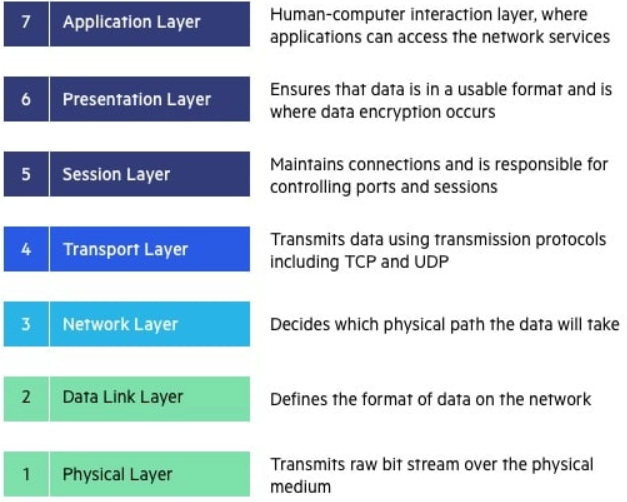
\includegraphics[width=0.6\linewidth]{../img/osi_model.png}

\subsubsection{Layer Abstraction}
\begin{itemize}
    \item Protocols enable an entity to interact with an entity at the same layer in another host
    \item \textbf{Service definitions:} provide functionality to an (N)-layer by an (N-1) layer
    \item Layer N exchange protocol data units (PDUs) with layer N protocol
    \item Each PDU contains a header and payload, the service data unit (SDU)
\end{itemize}
\textbf{Example PDU of L3:}\\
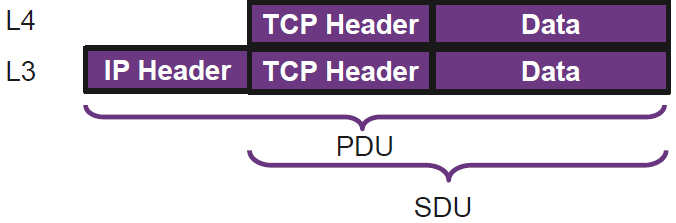
\includegraphics[width=0.6\linewidth]{../img/pdu.png}

\subsection{Layer 4 - Transport}
\subsubsection{TCP}
\begin{itemize}
    \item Reliable
    \item Ordered
    \item Window - capacity of receiver
    \item Checksum - 16bit
    \item TCP overhead: 20 bytes
    \item Tries to correct errors
\end{itemize}
\textbf{Connection establishment}
\begin{itemize}
    \item SYN, SYN-ACK, ACK
    \item Initiates TCP session: initial sequence number is random
\end{itemize}
\textbf{Connection termination}
\begin{itemize}
    \item FIN, ACK + FIN, ACK
    \item 3-way handshake
\end{itemize}
\textbf{Sequences and ACKs}
\begin{itemize}
    \item Identification each byte of data
    \item Order of the bytes: reconstruction
    \item Detecting lost data: RTO, DupACK
\end{itemize}
\textbf{Retransmission timeout}
\begin{itemize}
    \item If no ACK is received after timeout
\end{itemize}
\textbf{Flow control}
\begin{itemize}
    \item Sender is not overwhelming a receiver
    \item Back pressure
    \item Sliding window
    \item Congestion control
    \begin{itemize}
        \item Slow-start
        \item Congestion avoidance
    \end{itemize}
\end{itemize}

\subsubsection{TCP + TLS}
\textbf{TLS \textless 1.3}
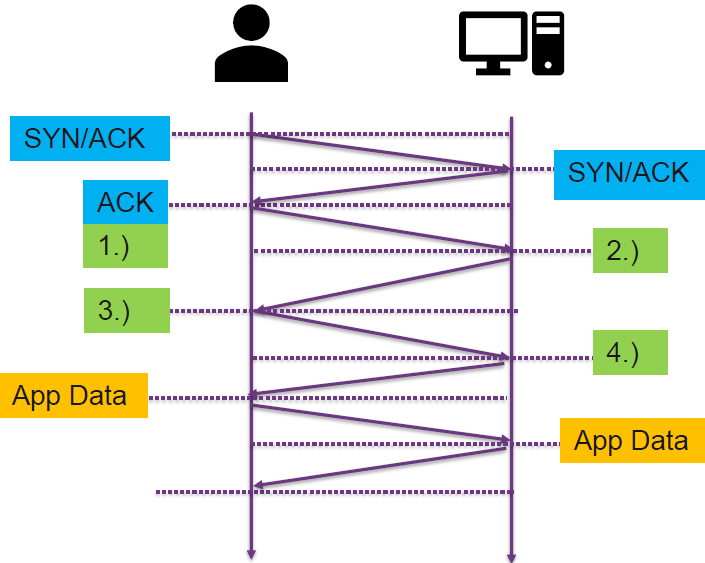
\includegraphics[width=0.7\linewidth]{../img/tcp_tls.png}
\begin{enumerate}
    \item client hello - lists crypto information, TLS version, ciphers/keys
    \item server hello - chosen cipher, session ID, random bytes, digital certificate
    \item Key exchange using random bytes, now client + server can calculate secret key
    \item finished - encrypted message
\end{enumerate}
3RTT until first byte\\
\textbf{TLS 1.3}
\begin{itemize}
    \item 1 RTT instead of 2
    \begin{enumerate}
        \item Client Hello, Key share
        \item Server Hello, Key share, Verify Certificate, Finished
    \end{enumerate}
    \item 0 RTT possible for previous connections (no perfect forward secrecy)
\end{itemize}

\subsubsection{QUIC}
\begin{itemize}
    \item 1 RTT (0 RTT for know connections)
    \item Built in security
\end{itemize}
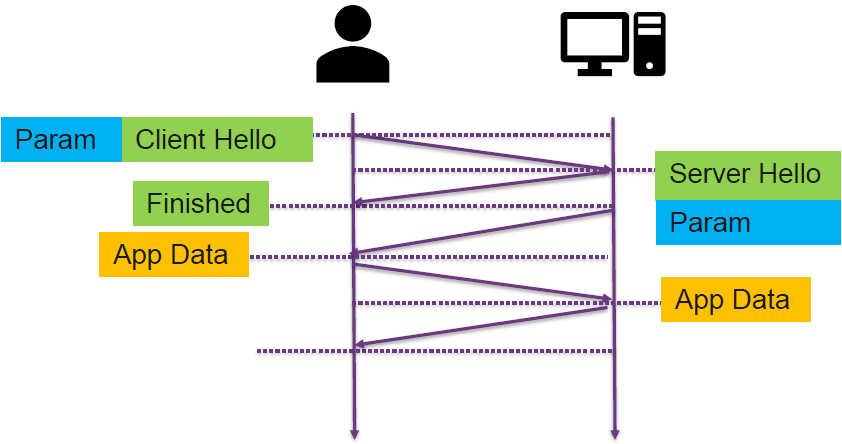
\includegraphics[width=0.8\linewidth]{../img/quic.png}
\begin{itemize}
    \item Multiplexing in HTTP/2
    \item QUIC can multiplex requests: one stream does not affect others
\end{itemize}

\subsubsection{UDP}
\begin{itemize}
    \item Used for DNS, streaming
    \item Simple connectionless communication model
    \item No guarantee
    \begin{itemize}
        \item Delivery
        \item Ordering
        \item Duplicate protection
    \end{itemize}
\end{itemize}

\subsubsection{SCTP - Stream Control Transmission Protocol}
\begin{itemize}
    \item Message based
    \item Allows data to be divided into multiple streams
    \item Syn cookies: Four-way handshake with a signed cookie
    \item Multi-homing multiple IP addresses of endpoints
\end{itemize}

    \end{multicols*}
\end{document}

























